\documentclass[12pt, a4paper]{article}

\usepackage{amsmath}
\usepackage{amssymb}
\usepackage{booktabs}
\usepackage{ctex}
\usepackage{enumitem}
\usepackage{fancyhdr}
\usepackage{float}
\usepackage{geometry}
\usepackage{graphicx}
\usepackage[colorlinks,linkcolor=black,anchorcolor=black,citecolor=blue,CJKbookmarks=True]{hyperref}
\usepackage{listings}
\usepackage{pifont}
\usepackage{url}
\usepackage{xcolor}

\definecolor{anhao-orange}{RGB}{255,140,0}
\definecolor{anhao-purple}{RGB}{148,0,211}
\definecolor{anhao-scarlet}{RGB}{178,34,34}
\definecolor{anhao-sky}{RGB}{30,144,255}
\definecolor{anhao-background}{RGB}{230,230,250}
\geometry{left=2cm,right=2cm,top=2cm,bottom=2cm}
\renewcommand{\contentsname}{\centering{\heiti\zihao{3}{Contents}}}

\begin{document}
	
\pagenumbering{Roman}
{\tableofcontents}
\newpage

\pagenumbering{arabic}

\section{Lecture 01 - 方程组的几何解释}
\pagestyle{fancy}
\lhead{}
\chead{Lecture 01 - 方程组的几何解释}
\rhead{}

\noindent${\mathbf{n}}$ linear equations, ${\mathbf{n}}$ unknowns
\begin{itemize}
	\item row picture
	\item column picture {\textcolor{anhao-scarlet}{\bf{$\star$}}}
	\item matrix form
\end{itemize}
\vspace{14pt}
\begin{math}
\left\{  
\begin{array}{rclrcl}
	2x & - & y  & = & 0 \\
	-x & + & 2y & = & 3
\end{array}  
\right.
\end{math}
\newline
\begin{math}
\begin{bmatrix}
	2  & -1 \\
	-1 & 2
\end{bmatrix}
\begin{bmatrix}
	x \\
	y
\end{bmatrix}
=
\begin{bmatrix}
	0 \\
	3
\end{bmatrix}
\end{math}
, i.e.
\newline
${\mathbf{A}}$ (matrix of coefficients) = 
\begin{math}
\begin{bmatrix}
	2  & -1 \\
	-1 & 2
\end{bmatrix}
\end{math}
, ${\mathbf{x}}$ (vector of unknowns) = 
\begin{math}
\begin{bmatrix}
	x \\
	y
\end{bmatrix}
\end{math}
, ${\mathbf{b}}$ = 
\begin{math}
\begin{bmatrix}
	0 \\
	3
\end{bmatrix}
\end{math}
, such that
\begin{displaymath}
{\mathbf{A}}{\mathbf{x}}={\mathbf{b}}
\end{displaymath}
\vspace{14pt}
what's the {\textcolor{anhao-scarlet}{\bf{row}}} picture?
\begin{center}
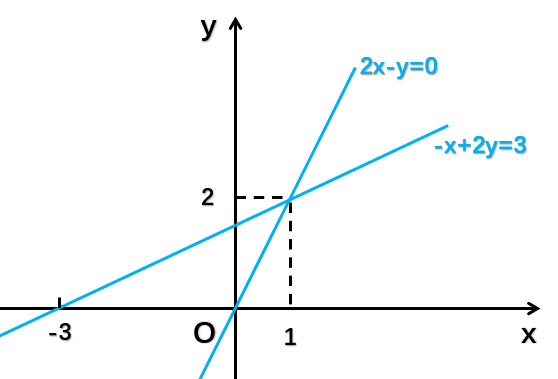
\includegraphics[width=0.4\textwidth]{figures/S1-1.png}
\end{center}
{\textcolor{anhao-purple}{to find the point that lies on both two lines}}
\newline
what's the {\textcolor{anhao-scarlet}{\bf{column}}} picture?
\newline
\begin{math}
x 
\begin{bmatrix}
	2 \\
	-1
\end{bmatrix}
+
y
\begin{bmatrix}
	-1 \\
	2
\end{bmatrix}
=
\begin{bmatrix}
	0 \\
	3
\end{bmatrix}
\end{math}
\begin{center}
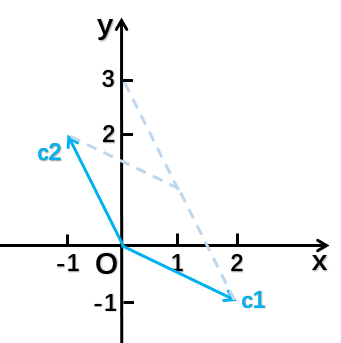
\includegraphics[width=0.3\textwidth]{figures/S1-2.png}
\end{center}
\begin{displaymath}
1{\overrightarrow{c_1}}+2{\overrightarrow{c_2}}={\overrightarrow{b}}
\end{displaymath}
{\textcolor{anhao-purple}{to find the linear combination of columns of ${\mathbf{A}}$, such that it equals ${\mathbf{b}}$}}
\vspace{14pt}
\newline
what linear combination gives ${\mathbf{b}}$?
\newline
what do all the linear combinations give?
\newline
what are all the possible, achievable right-hand sides be?
\vspace{14pt}
\newline
\begin{math}
\left\{  
\begin{array}{rclrclrclrcl}
	2x & - & y & & & = & 0 &{\bf{\textcolor{anhao-orange}{1}}}&\\
	-x & + & 2y & - & z & = & -1 &{\bf{\textcolor{anhao-orange}{2}}}&\\
	& -& 3y & + & 4z & = & 4 &{\bf{\textcolor{anhao-orange}{3}}}&
\end{array}  
\right.
\end{math}
\newline
\begin{math}
\left\{  
\begin{array}{rcl}
	&{\bf{\textcolor{anhao-orange}{1}}}&
\end{array}  
\right.
\end{math}
\quad : the plot of all the points that solve it are a plane
\newline
\begin{math}
\left\{  
\begin{array}{rcl}
	&{\bf{\textcolor{anhao-orange}{2}}}& \\
	&{\bf{\textcolor{anhao-orange}{3}}}&
\end{array}  
\right.
\end{math}
\quad : two planes meet at a line
\newline
\begin{math}
\left\{  
\begin{array}{rcl}
	&{\bf{\textcolor{anhao-orange}{1}}}& \\
	&{\bf{\textcolor{anhao-orange}{2}}}& \\
	&{\bf{\textcolor{anhao-orange}{3}}}&
\end{array}  
\right.
\end{math}
\quad : meet at a point
\newline
${\mathbf{A}}$ = 
\begin{math}
\begin{bmatrix}
	2  & -1 & 0 \\
	-1 & 2 & -1 \\
	0 & -3 & 4
\end{bmatrix}
\end{math}
, ${\mathbf{b}}$ =
\begin{math} 
\begin{bmatrix}
	0 \\
	-1\\
	4
\end{bmatrix}
\end{math}
\vspace{14pt}
\newline
what's the {\textcolor{anhao-scarlet}{\bf{row}}} picture?
\newline
{\textcolor{anhao-purple}{to find out all the points that satisfy all the equations}}
\newline
what's the {\textcolor{anhao-scarlet}{\bf{column}}} picture?
\newline
\begin{math}
x
\begin{bmatrix}
	2 \\
	-1\\
	0
\end{bmatrix}
 + y
\begin{bmatrix}
	-1 \\
	2\\
	-3
\end{bmatrix}
 + z
\begin{bmatrix}
	0 \\
	-1\\
	4
\end{bmatrix}
 = 
\begin{bmatrix}
	0 \\
	-1\\
	4
\end{bmatrix}
\end{math}
\vspace{14pt}
\newline
can I always solve ${\mathbf{A}}$${\mathbf{x}}$ = ${\mathbf{b}}$ for every right-hand side ${\mathbf{b}}$?
\newline
do the linear combinations of the columns fill 3-dimensional space?
\newline
{\textcolor{anhao-purple}{for this ${\mathbf{A}}$, the answer is {\bf{YES}} (non-singular, invertible)}}
\newline
{\textcolor{anhao-purple}{but for some others ${\mathbf{A}}$, the answer could be {\bf{NO}} (singular, not-invertible)}}
\vspace{14pt}
\newline
if the 3 columns all lie in the same plane, 
\newline
so I could solve it for some right-hand sides, when ${\overrightarrow{b}}$ is in the plane,
\newline
but most right-hand sides would be out of the plane and unreachable.
\vspace{14pt}
\newline
in some case, the combinations of ${\mathbf{n}}$ columns can only fill out ${\mathbf{m}}$-D ($m < n$)
\vspace{14pt}
\newline
\begin{math}
\begin{bmatrix}
	2 & 5 \\
	1 & 3 
\end{bmatrix}
\begin{bmatrix}
	1 \\
	2 
\end{bmatrix}
 = 
1
\begin{bmatrix}
	2 \\
	1 
\end{bmatrix}
 + 
2
\begin{bmatrix}
	5 \\
	3 
\end{bmatrix}
 = 
\begin{bmatrix}
	12 \\
	7 
\end{bmatrix}
\end{math}
\newline
${\mathbf{A}}$${\mathbf{x}}$ means: ${\mathbf{A}}$${\mathbf{x}}$ is a combination of columns of ${\mathbf{A}}$

\newpage
\section{Lecture 02 - 矩阵消元}
\pagestyle{fancy}
\lhead{}
\chead{Lecture 02 - 矩阵消元}
\rhead{}

\noindent when solving equations-system, 
\newline
{\bf{Elimination}}, if it succeeds, it gets the answer.
\newline
It's always good to ask how could it fail.
\vspace{14pt}
\newline
\begin{math}
	\left\{  
	\begin{array}{rclrclrcl}
		x & + & 2y & + & z & = & 2 \\
		3x & + & 8y & + & z & = & 12 \\
		& & 4y & + & z & = & 2 
	\end{array}  
	\right.
\end{math}
\vspace{14pt}
\newline
\begin{math}
	\begin{bmatrix}
		{\bf{\textcolor{anhao-sky}{\mathop{1}\limits_{first-pivot}}}} & 2 & 1 \\
		3 & 8 & 1 \\
		0 & 4 & 1
	\end{bmatrix}
	\xrightarrow[row_3 - 0 \times row_1]{row_2 - 3 \times row_1}
	\begin{bmatrix}
		1 & 2 & 1 \\
		0 & {\bf{\textcolor{anhao-sky}{\mathop{2}\limits_{second-pivot}}}} & -2 \\
		0 & 4 & 1
	\end{bmatrix}
	\xrightarrow[]{row_3 - 2 \times row_2}
	\begin{bmatrix}
		1 & 2 & 1 \\
		0 & 2 & -2 \\
		0 & 0 & {\bf{\textcolor{anhao-sky}{\mathop{5}\limits_{third-pivot}}}}
	\end{bmatrix}
\end{math}
\newline
{\textcolor{anhao-scarlet}{pivots can {\bf{NOT}} be 0 !}}
\newline
if there is a 0 in the pivot position, then try to switch lines
\newline
if 0 is in the pivot position and no place to exchange, then failure
\vspace{14pt}
\newline
let's bring the right-hand side in (Augmented Matrix)
\newline
\begin{math}
	\left[
	\begin{array}{ccc|c}
		1 & 2 & 1 & 2 \\
		3 & 8 & 1 & 12 \\
		0 & 4 & 1 & 2
	\end{array}
	\right]
	\longrightarrow
	\left[
	\begin{array}{ccc|c}
		1 & 2 & 1 & 2 \\
		0 & 2 & -2 & 6 \\
		0 & 4 & 1 & 2
	\end{array}
	\right]
	\longrightarrow
	\left[
	\begin{array}{ccc|c}
		1 & 2 & 1 & 2 \\
		0 & 2 & -2 & 6 \\
		0 & 0 & 5 & -10
	\end{array}
	\right]
	\Rightarrow
	\left\{  
	\begin{array}{rclrclrcl}
		x & + & 2y & + & z  & = & 2 \\
		  &   & 2y & - & 2z & = & 6  \\
		  &   &    &   & 5z & = & -10  
	\end{array}  
	\right.
\end{math}
\newline
by back-substitution: 
\begin{math}
	x = 2, y = 1, z = -2
\end{math}
\vspace{14pt}
\newline
{\bf{"elimination matrices"}}
\vspace{14pt}
\newline
\begin{math}
	\begin{bmatrix}
		{\textcolor{anhao-orange}{\vdots}} & {\textcolor{green}{\vdots}} & {\textcolor{purple}{\vdots}} \\
		{\textcolor{anhao-orange}{col_1}} & {\textcolor{green}{col_2}} & {\textcolor{purple}{col_3}} \\
		{\textcolor{anhao-orange}{\vdots}} & {\textcolor{green}{\vdots}} & {\textcolor{purple}{\vdots}}
	\end{bmatrix}
	\begin{bmatrix}
		1 \\
		2 \\
		3
	\end{bmatrix}
	 = 
	\begin{bmatrix}
		\ \\
		\ \\
		\ 
	\end{bmatrix}
	 = 
	1 \times {\textcolor{anhao-orange}{col_1}} + 2 \times {\textcolor{green}{col_2}} + 3 \times {\textcolor{purple}{col_3}}
\end{math}
\newline
{\textcolor{anhao-purple}{the result of multiplying a matrix by some vectors, is a combination of columns of the matrix}}
\vspace{14pt}
\newline
\begin{math}
	\begin{bmatrix}
		1 & 2 & 7
	\end{bmatrix}
	\begin{bmatrix}
		{\textcolor{anhao-orange}{\cdots}} & {\textcolor{anhao-orange}{row_1}} & {\textcolor{anhao-orange}{\cdots}} \\
		{\textcolor{green}{\cdots}} & {\textcolor{green}{row_2}} & {\textcolor{green}{\cdots}} \\
		{\textcolor{purple}{\cdots}} & {\textcolor{purple}{row_3}} & {\textcolor{purple}{\cdots}}
	\end{bmatrix}
	 = 
	\begin{bmatrix}
		\ & \ & \
	\end{bmatrix}
	 = 
	\begin{array}{rcl}
		1 & \times &  {\textcolor{anhao-orange}{row_1}} \\
		 & + & \\
		2 & \times & {\textcolor{green}{row_2}} \\
		 & + & \\
		7 & \times & {\textcolor{purple}{row_3}}
	\end{array}
\end{math}
\newline
{\textcolor{anhao-purple}{the product of a row times a matrix, is a combination of rows of the matrix}}
\vspace{14pt}
\newline
when we do matrix multiplication, keep your eye on what it is doing with the whole vectors
\vspace{14pt}
\newline
what does the matrix, which can subtract $3 \times row_1$ from $row_2$ look like?
\newline
i.e. 
\begin{math}
	\begin{bmatrix}
		? & ? & ? \\
		? & ? & ? \\
		? & ? & ? 
	\end{bmatrix}
	\begin{bmatrix}
		1 & 2 & 1 \\
		3 & 8 & 1 \\
		0 & 4 & 1 
	\end{bmatrix}
	 = 
	\begin{bmatrix}
		1 & 2 & 1 \\
		0 & 2 & -2 \\
		0 & 4 & 1 
	\end{bmatrix}
\end{math}
\newline
\begin{math}
	\begin{bmatrix}
		? & ? & ? \\
		? & ? & ? \\
		? & ? & ? 
	\end{bmatrix}
	\\
	\xrightarrow[]{as \ R_1 = {\textcolor{anhao-scarlet}{\bf{1}}} \times row_1 + {\textcolor{anhao-scarlet}{\bf{0}}} \times row_2 + {\textcolor{anhao-scarlet}{\bf{0}}} \times row_3}
	\begin{bmatrix}
		1 & 0 & 0 \\
		? & ? & ? \\
		? & ? & ? 
	\end{bmatrix}
	\\
	\xrightarrow[]{as \ R_3 = {\textcolor{anhao-scarlet}{\bf{0}}} \times row_1 + {\textcolor{anhao-scarlet}{\bf{0}}} \times row_2 + {\textcolor{anhao-scarlet}{\bf{1}}} \times row_3}
	\begin{bmatrix}
		1 & 0 & 0 \\
		? & ? & ? \\
		0 & 0 & 1 
	\end{bmatrix}
	\\
	\xrightarrow[]{as \ R_2 = {\textcolor{anhao-scarlet}{\bf{-3}}} \times row_1 + {\textcolor{anhao-scarlet}{\bf{1}}} \times row_2 + {\textcolor{anhao-scarlet}{\bf{0}}} \times row_3}
	\begin{bmatrix}
		1 & 0 & 0 \\
		-3 & 1 & 0 \\
		0 & 0 & 1 
	\end{bmatrix}
\end{math}
\newline
\begin{math}
	\begin{bmatrix}
		1 & 0 & 0 \\
		-3 & 1 & 0 \\
		0 & 0 & 1 
	\end{bmatrix}
\end{math}
: elementary matrix (初等矩阵)
\newline
${\mathbf{E_{i,j}}}$ means it's the matrix that we use to fix the (i, j) position
\newline
e.g. 
\begin{math}
	\begin{bmatrix}
		? & ? & ? \\
		? & ? & ? \\
		? & ? & ? 
	\end{bmatrix}
	\xrightarrow[]{R_1=row_1}
	\begin{bmatrix}
		1 & 0 & 0 \\
		? & ? & ? \\
		? & ? & ? 
	\end{bmatrix}
	\xrightarrow[]{R_2=row_2}
	\begin{bmatrix}
		1 & 0 & 0 \\
		0 & 1 & 0 \\
		? & ? & ? 
	\end{bmatrix}
	\xrightarrow[]{R_3 = row_3 - 2 \times row_2}
	\begin{bmatrix}
		1 & 0 & 0 \\
		0 & 1 & 0 \\
		0 & -2 & 1 
	\end{bmatrix}
	 = 
	E_{3,2}
\end{math}
\vspace{14pt}
\newline
in elimination, we can use an elementary matrix to describe the change in each step
\vspace{14pt}
\newline
the next point in this lecture is to put these steps together, into a matrix that does these steps all in sequence, in another words, how could I create the matrix that does the whole job at once? i.e.
\begin{displaymath}
	{\mathbf{E_{3,2}}}({\mathbf{E_{2,1}}}{\mathbf{A}}) = {\mathbf{U}} \Longleftrightarrow {\mathbf{\boxed{?}}}{\mathbf{A}} = {\mathbf{U}}
\end{displaymath}
\vspace{14pt}
\newline
{\bf{Associative Law}}
\begin{displaymath}
	({\mathbf{A}}{\mathbf{B}}){\mathbf{C}} = {\mathbf{A}}({\mathbf{B}}{\mathbf{C}})
\end{displaymath}
\vspace{14pt}
\newline
permutation(置换): 
\begin{itemize}
	\item exchange rows, e.g.
	\par 
	\begin{math}
		\begin{bmatrix}
			? & ? \\
			? & ?
		\end{bmatrix}
		\begin{bmatrix}
			a & b \\
			c & d
		\end{bmatrix}
		 = 
		\begin{bmatrix}
			c & d \\
			a & b
		\end{bmatrix}
	\end{math}
	\par ${\mathbf{P}}$ = 
	\begin{math}
		\begin{bmatrix}
			0 & 1 \\
			1 & 0
		\end{bmatrix}
	\end{math}
	is to exchange $row_1$ and $row_2$
	\item exchange columns, e.g.
	\par 
	\begin{math}
		\begin{bmatrix}
			a & b \\
			c & d
		\end{bmatrix}
		\begin{bmatrix}
			? & ? \\
			? & ?
		\end{bmatrix}
		= 
		\begin{bmatrix}
			b & a \\
			d & c
		\end{bmatrix}
	\end{math}
	\par ${\mathbf{P}}$ = 
	\begin{math}
		\begin{bmatrix}
			0 & 1 \\
			1 & 0
		\end{bmatrix}
	\end{math}
	is to exchange $col_1$ and $col_2$
\end{itemize}
\vspace{14pt}
{\textcolor{anhao-purple}{when I multiply a matrix on the left, I am doing row operations}}
\newline
{\textcolor{anhao-purple}{if I want to do column operations, I should put a matrix on the right}}
\vspace{14pt}
\newline
if ${\mathbf{\boxed{?}}}{\mathbf{A}} = {\mathbf{U}}$, then how can I "from ${\mathbf{U}}$ back to ${\mathbf{A}}$"?
\newline
this is about reversing steps, invertible, $\cdots$
\newline
\begin{math}
	\begin{bmatrix}
		1 & 0 & 0 \\
		-3 & 1 & 0 \\
		0 & 0 & 1
	\end{bmatrix}^{-1}
	 = 
	\begin{bmatrix}
		1 & 0 & 0 \\
		3 & 1 & 0 \\
		0 & 0 & 1
	\end{bmatrix}
\end{math}
\newline
"what steps can get me back?"
\newline
"what matrix can bring me back?"

\newpage
\section{Lecture 03 - 乘法和逆矩阵}
\pagestyle{fancy}
\lhead{}
\chead{Lecture 03 - 乘法和逆矩阵}
\rhead{}

\noindent
key words:
\begin{itemize}
	\item matrix multiplication (4 ways)
	\item inverse of ${\mathbf{A}}$, ${\mathbf{AB}}$, ${\mathbf{A^{T}}}$
	\item Gauss-Jordan, to find ${\mathbf{A^{-1}}}$
\end{itemize}
\vspace{14pt}
\begin{math}
	\underbrace{
		\begin{bmatrix}
			\ \ & \ & \ & \ \ \\
			\ \ & \ & \ & \ \ \\
			\ \ & \ & \ & \ \ 
		\end{bmatrix}
	}_{\mathbf{A}}
	\underbrace{
		\begin{bmatrix}
			\ \ & \ & \ \ \\
			\ \ & \ & \ \ \\
			\ \ & \ & \ \ \\
			\ \ & \ & \ \ 
		\end{bmatrix}
	}_{\mathbf{B}}
	 = 
	\underbrace{
		\begin{bmatrix}
			\ \ & \ & \ \ \\
			\ \ & c_{i,j} & \ \ \\
			\ \ & \ & \ \ 
		\end{bmatrix}
	}_{\mathbf{C=AB}}
\end{math}
\newline
$c_{i,j}$ comes from $row_i$ of ${\mathbf{A}}$ and $col_j$ of ${\mathbf{B}}$
\newline
e.g.
\par 
\begin{math}
	\begin{aligned}
		c_{3,4} &= 
		\begin{bmatrix}
			\ & \ & \ & \ & \ \\
			\ & {\textcolor{anhao-orange}{row_3}} & {\textcolor{anhao-orange}{of}} & {\textcolor{anhao-orange}{\mathbf{A}}} & \ \\
			\ & \ & \ & \ & \ 
		\end{bmatrix}
		\begin{bmatrix}
			\ & \ & \ \\
			\ & {\textcolor{anhao-purple}{col_4}} & \ \\
			\ & {\textcolor{anhao-purple}{of}} & \ \\
			\ & {\textcolor{anhao-purple}{\mathbf{B}}} & \ \\
			\ & \ & \
		\end{bmatrix} \\
				&= a_{3,1}b_{1,4} + a_{3,2}b_{2,4} + \cdots + a_{3,i}b_{i,4} + \cdots + a_{3,n}b_{n,4} \\
				&= \sum_{k=1}^{n}a_{3,k}b_{k,4}
	\end{aligned}
\end{math}
\vspace{14pt}
\newline
{\textcolor{anhao-scarlet}{the number of columns of ${\mathbf{A}}$ has to match the number of rows of ${\mathbf{B}}$}
\begin{displaymath}
	{\mathbf{A}}_{m \times n}{\mathbf{B}}_{n \times p} = {\mathbf{C}}_{m \times p}
\end{displaymath}
\vspace{14pt}
the matrix times the $n^{\text{th}}$ column is the $n^{\text{th}}$ column of the answer
\begin{center}
	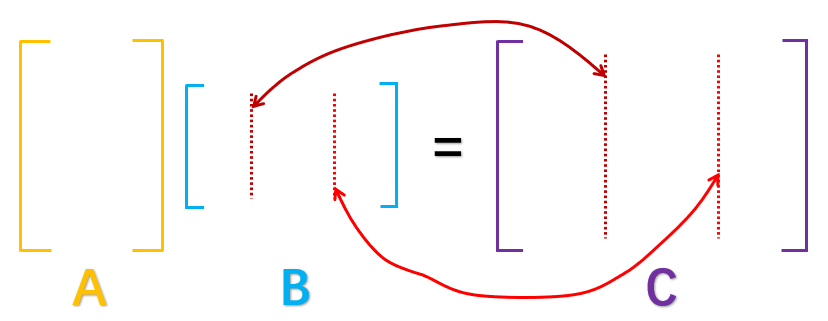
\includegraphics[scale=0.5]{figures/S3-1.png}
\end{center}
so I could think of multiplying a matrix by a vector, side by side
\newline
I can just think of having several columns, multiplying by ${\mathbf{A}}$, and getting the columns of answer
\vspace{14pt}
\newline
{\textcolor{anhao-purple}{the columns of ${\mathbf{C}}$ are combinations of columns of ${\mathbf{A}}$}}
\newline
$\Longleftrightarrow$ every column of ${\mathbf{C}}$ is a combination of columns of ${\mathbf{A}}$, and numbers in ${\mathbf{B}}$ tell me what the combination is
\newline
in the same way, {\textcolor{anhao-purple}{the rows of ${\mathbf{C}}$ are combinations of rows of ${\mathbf{B}}$}}
\vspace{14pt}
\newline
what about " 
\begin{math}
	\underbrace{col \ \ of \ \ {\mathbf{A}}}_{m \times 1}
	\quad \times \quad
	\underbrace{row \ \ of \ \ {\mathbf{B}}}_{1 \times p}
\end{math}
 "?
\newline
e.g.
\par 
\begin{math}
	\begin{bmatrix}
		2 \\
		3 \\
		4
	\end{bmatrix}
	\begin{bmatrix}
		1 & 6
	\end{bmatrix}
	 = 
	\begin{bmatrix}
		2 & 12 \\
		3 & 18 \\
		4 & 24 
	\end{bmatrix}
\end{math}
\par 
\begin{math}
	\begin{bmatrix}
		2 & 7 \\
		3 & 8 \\
		4 & 9 
	\end{bmatrix}
	\begin{bmatrix}
		1 & 6 \\
		0 & 0 
	\end{bmatrix}
	 = 
	\begin{bmatrix}
		2 \\
		3 \\
		4
	\end{bmatrix}
	\begin{bmatrix}
		1 & 6
	\end{bmatrix}
	 + 
	\begin{bmatrix}
		7 \\
		8 \\
		9
	\end{bmatrix}
	\begin{bmatrix}
		0 & 0
	\end{bmatrix}
\end{math}
\newline
\begin{math}
	\begin{aligned}
		{\mathbf{AB}} &= {\text{sum of}} \ \ (col_i \ of \ {\mathbf{A}}) \times (row_i \ of \ {\mathbf{B}}) \\
		&= \sum_{i=1}^{n}(col_i \ of \ {\mathbf{A}}) \times (row_i \ of \ {\mathbf{B}})
	\end{aligned}
\end{math}
\vspace{14pt}
\newline
{\textcolor{anhao-purple}{the row space}} for 
\begin{math}
	\begin{bmatrix}
		2 & 12 \\
		3 & 18 \\
		4 & 24
	\end{bmatrix}
\end{math}
, which is like all combinations of the rows, is the line through the row-vector 
\begin{math}
	\begin{bmatrix}
		1 & 6
	\end{bmatrix}
\end{math}, the same to {\textcolor{anhao-purple}{the column space}}
\vspace{14pt}
\newline
you could also cut the matrix into blocks and do the multiplication by blocks, i.e.
\begin{displaymath}
	\underbrace{
		\left[
		\begin{array}{c|c}
			{\mathbf{A_1}} & {\mathbf{A_2}} \\
			\hline
			{\mathbf{A_3}} & {\mathbf{A_4}}
		\end{array}
		\right]
	}_{{\mathbf{A}}}
	\underbrace{
		\left[
		\begin{array}{c|c}
			{\mathbf{B_1}} & {\mathbf{B_2}} \\
			\hline
			{\mathbf{B_3}} & {\mathbf{B_4}}
		\end{array}
		\right]
	}_{{\mathbf{B}}}
	 = 
	\underbrace{
		\left[
		\begin{array}{c|c}
			{\mathbf{A_1B_1+A_2B_3}} & {\mathbf{A_1B_2+A_2B_4}} \\
			\hline
			{\mathbf{A_3B_1+A_4B_3}} & {\mathbf{A_3B_2+A_4B_4}}
		\end{array}
		\right]
	}_{{\mathbf{AB}}}
\end{displaymath}
\vspace{14pt}
\newline
\noindent{\textcolor{anhao-purple}{Inverses (square matrices)}}
\newline
not all matrices have inverses, if a matrix is square, is it invertible or not?
\newline
if ${\mathbf{A}}$ is invertible, non-singular, then
\begin{displaymath}
	{\mathbf{A^{-1}}}{\mathbf{A}} = {\mathbf{I}} = {\mathbf{A}}{\mathbf{A^{-1}}}
\end{displaymath}
in singular case, no inverse!
\newline
e.g.
\par 
\begin{math}
	{\mathbf{A}} = 
	\begin{bmatrix}
		1 & 3 \\
		2 & 6
	\end{bmatrix}
\end{math}
\par thinking about columns here, if I multiply ${\mathbf{A}}$ by some other matrices, the columns of the results are all multiples of 
\begin{math}
	\begin{bmatrix}
		1 \\
		2
	\end{bmatrix}
\end{math}
, so no way to get the identity matrix ${\mathbf{I}}$
\par there is another more important reason
\par a square matrix has no inverse if I can find a vector ${\mathbf{x}}$ such that ${\mathbf{A}}{\mathbf{x}} = {\mathbf{0}}$ and ${\mathbf{x}} \neq {\mathbf{0}}$
\par but 
\par \qquad
\begin{math}
	\begin{bmatrix}
		1 & 3 \\
		2 & 6
	\end{bmatrix}
	\begin{bmatrix}
		3 \\
		-1
	\end{bmatrix}
	 = 
	\begin{bmatrix}
		0 \\
		0
	\end{bmatrix}
\end{math}
\vspace{14pt}
\newline
{\textcolor{anhao-scarlet}{the matrix can't have an inverse if some columns give no contribution!}}
\vspace{14pt}
\newline
because
\par if 
\begin{math}
	{\mathbf{A}} = 
	\begin{bmatrix}
		1 & 3 \\
		2 & 6
	\end{bmatrix}
\end{math}
 has an inverse, named ${\mathbf{A^{-1}}}$, then 
\begin{math}
	{\mathbf{A^{-1}}}{\mathbf{A}}
	\begin{bmatrix}
		3 \\
		-1
	\end{bmatrix}
	 = 
	{\mathbf{A^{-1}}}
	\begin{bmatrix}
		0 \\
		0
	\end{bmatrix}
\end{math}
, 
\par 
and meanwhile, 
\begin{math}
	{\mathbf{A^{-1}}}{\mathbf{A}}
	\begin{bmatrix}
		3 \\
		-1
	\end{bmatrix}
	= 
	{\mathbf{I}}
	\begin{bmatrix}
		3 \\
		-1
	\end{bmatrix}
	 = 
	\begin{bmatrix}
		3 \\
		-1
	\end{bmatrix}
\end{math}
, 
\par
so that 
\begin{math}
	\begin{bmatrix}
		3 \\
		-1
	\end{bmatrix}
	 = 
	\begin{bmatrix}
		0 \\
		0
	\end{bmatrix}
\end{math}
, which is not True
\vspace{14pt}
\newline
{\textcolor{anhao-scarlet}{our conclusion is that for non-invertible/singular matrices, some combinations of their columns give the zero column}}
\vspace{14pt}
\newline
let's take a matrix that does have an inverse for example
\newline
e.g.
\par 
\begin{math}
	{
		\underbrace{
			\begin{bmatrix}
				1 & 3 \\
				2 & 7
			\end{bmatrix}
		}_{\mathbf{A}}
	}
	{
		\underbrace{
			\begin{bmatrix}
				a & b \\
				c & d
			\end{bmatrix}
		}_{\mathbf{A^{-1}}}
	}
	 = 
	{
		\underbrace{
			\begin{bmatrix}
				1 & 0 \\
				0 & 1
			\end{bmatrix}
		}_{\mathbf{I}}
	}
\end{math}
\par then
\begin{math}
	\left\{  
	\begin{array}{rcl}
		{\mathbf{A}}
		\begin{bmatrix}
			a \\
			b 
		\end{bmatrix}
		& = & 
		\begin{bmatrix}
		 	1 \\
		 	0 
		\end{bmatrix} 
		\\
		{\mathbf{A}}
		\begin{bmatrix}
			c \\
			d 
		\end{bmatrix}
		& = & 
		\begin{bmatrix}
		 	0 \\
		 	1 
		\end{bmatrix}
	\end{array}  
	\right.
\end{math}
\newline
generally, 
\begin{displaymath}
	{\mathbf{A}} \cdot (col_j \ of \ {\mathbf{A^{-1}}}) = (col_j \ of \ {\mathbf{I}})
\end{displaymath}
\vspace{14pt}
\newline
then how to solve the inverse for an invertible matrix?
\newline
here is the Gauss-Jordan idea, to solve two equations at once
\newline
\begin{math}
	\left\{  
	\begin{array}{rcl}
		\begin{bmatrix}
			1 & 3 \\
			2 & 7 
		\end{bmatrix}
		\begin{bmatrix}
			a \\
			b 
		\end{bmatrix}
		& = & 
		\begin{bmatrix}
			1 \\
			0 
		\end{bmatrix} 
		\\
		\begin{bmatrix}
			1 & 3 \\
			2 & 7 
		\end{bmatrix}
		\begin{bmatrix}
			c \\
			d 
		\end{bmatrix}
		& = & 
		\begin{bmatrix}
			0 \\
			1 
		\end{bmatrix}
	\end{array}  
	\right.
\end{math}
\newline
"solve them together!"
\newline
\begin{math}
	\underbrace{
		\left[
		\begin{array}{cc|cc}
			1 & 3 & 1 & 0 \\
			2 & 7 & 0 & 1
		\end{array}
		\right]
	}_{
		\left[
		\begin{array}{c|c}
			{\mathbf{A}} & {\mathbf{I}}
		\end{array}
		\right]
	}
	\rightarrow
	\left[
	\begin{array}{cc|cc}
		1 & 3 & 1 & 0 \\
		0 & 1 & -2 & 1
	\end{array}
	\right]
	\rightarrow
	\underbrace{
		\left[
		\begin{array}{cc|cc}
			1 & 0 & 7 & -3 \\
			0 & 1 & -2 & 1
		\end{array}
		\right]
	}_{
		\left[
		\begin{array}{c|c}
			{\mathbf{I}} & {\mathbf{A^{-1}}}
		\end{array}
		\right]
	}
\end{math}
\newline
把单位矩阵当成草稿纸,记录下对左侧矩阵的变换
\newline
相当于左右两边同时乘上逆矩阵,当左边变成单位矩阵时,右边即是该逆矩阵
\newline
i.e.
\par
\begin{math}
	\begin{aligned}
		{\mathbf{E}}_{i_1,j_1}
		{\mathbf{E}}_{i_2,j_2}
		\cdots
		{\mathbf{E}}_{i_n,j_n}
		\left[
		\begin{array}{c|c}
			{\mathbf{A}} & {\mathbf{I}}
		\end{array}
		\right]
		&= 
		\left[
		\begin{array}{c|c}
			{{\mathbf{E}}_{i_1,j_1}{\mathbf{E}}_{i_2,j_2}\cdots{\mathbf{E}}_{i_n,j_n}{\mathbf{A}}} & {{\mathbf{E}}_{i_1,j_1}{\mathbf{E}}_{i_2,j_2}\cdots{\mathbf{E}}_{i_n,j_n}{\mathbf{I}}}
		\end{array}
		\right]
		\\
		&= 
		\left[
		\begin{array}{c|c}
			{\mathbf{I}} & 
			{\mathbf{E}}_{i_1,j_1}{\mathbf{E}}_{i_2,j_2}\cdots{\mathbf{E}}_{i_n,j_n}
		\end{array}
		\right]
	\end{aligned}
\end{math}
\par
then 
\begin{math}
	{\mathbf{A^{-1}}} = {\mathbf{E}}_{i_1,j_1}{\mathbf{E}}_{i_2,j_2}\cdots{\mathbf{E}}_{i_n,j_n}
\end{math}
\par 注:
\par\qquad 
\begin{math}
	{\mathbf{E}}_{i_t,j_t}
	\left[
	\begin{array}{c|c}
		{\mathbf{A}} & {\mathbf{I}}
	\end{array}
	\right]
\end{math}
,即对
\begin{math}
	\left[
	\begin{array}{c|c}
		{\mathbf{A}} & {\mathbf{I}}
	\end{array}
	\right]
\end{math}
做行变换
$\Longleftrightarrow$
对${\mathbf{A}}$与${\mathbf{I}}$同时、做同样的行变换
\par\qquad 
同理,可以对
\begin{math}
	\left[
	\begin{array}{c}
		{\mathbf{A}} \\
		\hline
	    {\mathbf{I}}
	\end{array}
	\right]
\end{math}
做列变换,求得${\mathbf{A^{-1}}}$
\end{document}